\documentclass{article}
\usepackage{graphicx}
\usepackage{Sweave}
\begin{document}
\Sconcordance{concordance:FinalProjectPingTimes.tex:FinalProjectPingTimes.Rnw:%
1 2 1 1 0 24 1 1 12 2 1 1 2 5 0 1 2 5 1 1 2 5 0 1 2 8 1 1 2 1 0 1 1 4 0 %
1 2 5 1 1 2 1 0 1 1 4 0 1 2 7 1 1 2 8 0 1 2 4 1 1 2 8 0 1 2 2 1 1 12 4 %
0 1 2 2 1 1 18 1 1 1 2 6 0 1 1 5 0 1 1 5 0 1 2 6 0 1 1 7 0 1 2 23 1}

\title{Estimation of True Difference in Internet Latency Between Charter Internet and Kalamazoo College ISP}
\author{Daniel Michelin, Erik Hartig, and Nicholas Swain}
\maketitle
\begin{abstract}
In this paper we estimate the true $\mu$ of the difference between ping times between Kalamazoo College and a residence within a mile located at 416 Oak St. We hypothesize that a significant difference in latency as measured by ping times is likely indicative of substantially different network architecture. 
\end{abstract}
\section{Introduction}
A good network connection can be evaluated in a number of ways. One way it can be looked at is through a measure called latency, which is the time taken to send a packet of information from one point to another. A packet of information is a fundamental unit of data sent over packet-controlled networks such as the Internet. Another common way is to look at bandwidth, or the amount of data that can be transmitted at a single point of time. The difference between the two can be thought as analgous to delivering mail by hand. If a single packet can be thought of as a letter, then the latency can be thought of as the time it takes for the mail-person to get a single letter from point A to point B. Bandwidth by the same analogy can be thought of the number of letters that the mailperson is transmitting at a particular time. While it can be easy to confuse the two, a packet can have a low bandwidth and high latency, and vice versa. In the former case that mailperson could be transmitting mail using a high speed motorcycle: not much mail can go through at any particular time, but the mail that is on the network is rapidly transmitted. The latter case could be transmitting mail through a large truck: high capacity, low speed. Although TCP/IP, the fundamental architecture of the internet, has a maximum packet size of 64 Kilobytes the realistic maximum size of a packet is capped out usually at 1500 bytes, the maximum size of an ethernet packet. Most consumer internet connections run through ethernet, meaning that a single packet of information typically has a negligible effect on a network. Bandwidth is typically effected by traffic on the network, latency is not unless if the bandwidth has run out on a network. On most consumer internet plans the various tiers of paid internet service have the same latency, and a differing latency between two networks often means that there is something physically different between the networks, such as a shorter physical connection or faster wires (DSL vs Fiber optic for instance.). Ping is a software utility tests the network latency of a single packet and is featured across all popular operating systems. Our hypothesis is that there is a difference in means between Kalamazoo College's and the Oak Street residence's latencies as measured by ping time to google.com. We can state this as:


\begin{centering}
$H_0: \mu_{kzoo} = \mu_{oak}$ \\
\end{centering}

\begin{centering}
$H_A: \mu_{kzoo} \ne \mu_{oak}$ \\
\end{centering}


The alternative hypothesis is indicative of two things, the first being that the network itself is faster, and/or possibly that the network follows a different path to get to google.
\section{Methods}
We collected four datasets, two to estimate population parameters and two for exploratory data analysis. Samples collected from Kalamazoo College and the Oak Street residence that are used to estimate the $\mu$ of the population of the difference in means were collected at approximately the same time (within seconds of each other) to control for overall network business. These times were conducted by two laptops running a sample collection script in python that is included in the appendix. The Oak Street residence was chosen because of it's short distance from Kalamazoo College to minimize the impact of absolute physical distance being a factor in the latency difference, as large discrepancies in physical distance alone can contribute to wide differences in latency times, such as comparing a laptop in Google's headquarter's latency to google compared to a laptop in a Starbucks in Kalamazoo, MI. The script calls the Windows ping command line utility then parses the output for the correct value. The script takes 36 samples at an interval of 5 minutes each and records the location and latency. Laptops tested used the same Wifi chip to account for possible increase in latency there. Latency from router distance was controlled by being approximately the same distance from each one (about 6 feet with line of sight). Latency derived from the router itself is negligable. Tests were independent as a single packet is highly unlikely to impact the network in a measurable way.
\section{Results}
\begin{figure}
\centering
\caption{Histogram of observed Kalamazoo College Ping Times}
\begin{Schunk}
\begin{Sinput}
> hist(KalamazooCollege)
\end{Sinput}
\end{Schunk}
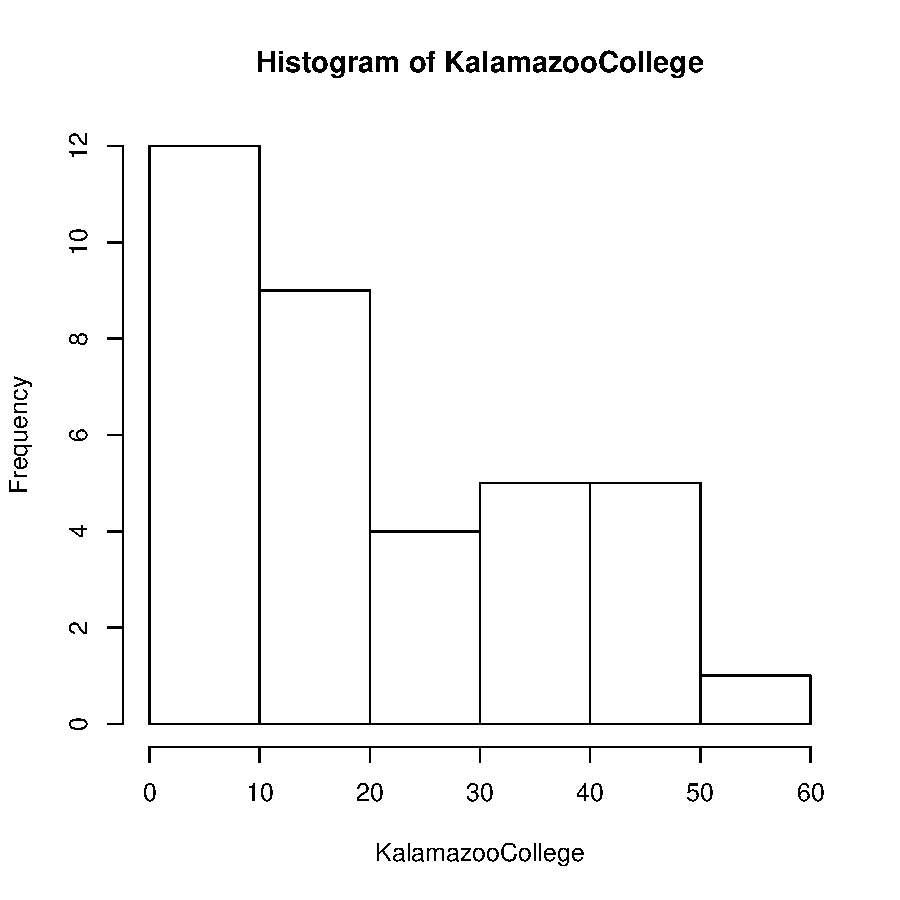
\includegraphics{FinalProjectPingTimes-002}
\label{fig:kzootimes}
\end{figure}

\begin{figure}
\centering
\caption{Histogram of observed Oak Street residence Ping Times}
\begin{Schunk}
\begin{Sinput}
> hist(PersonalResidence)
\end{Sinput}
\end{Schunk}
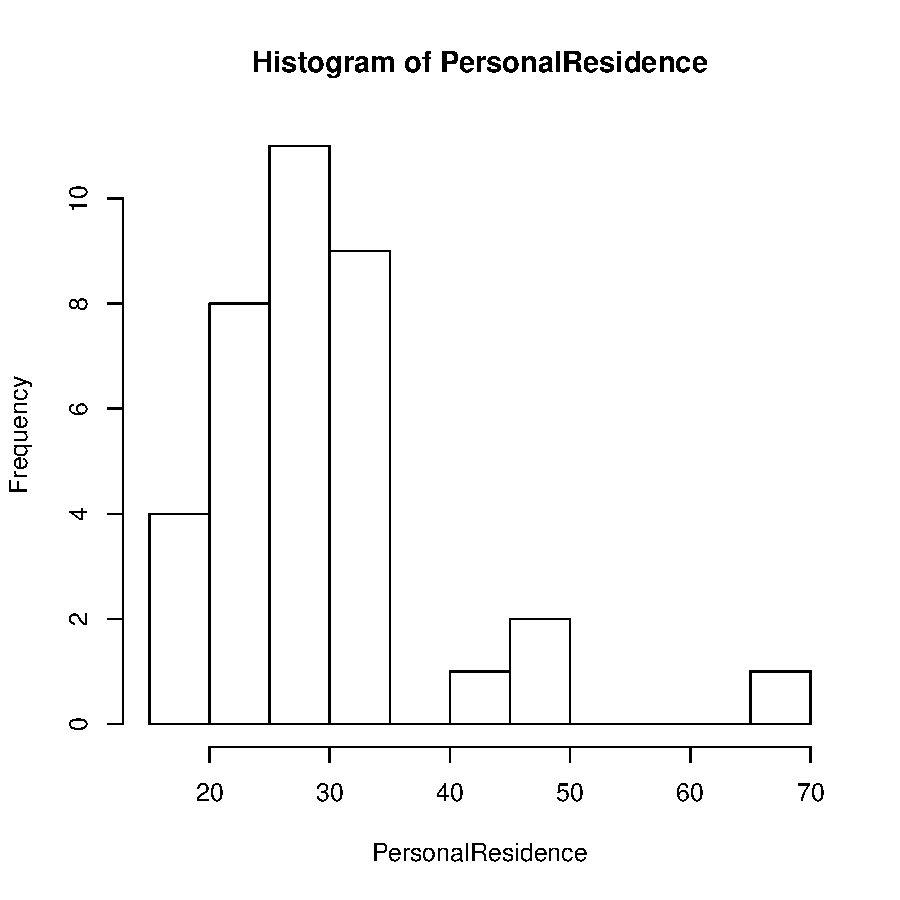
\includegraphics{FinalProjectPingTimes-003}
\label{fig:personalresidencetimes}
\end{figure}
To get an idea of the sampling distributions we look at histograms of the two distributions and summary descriptions of each. In figures \ref{fig:kzootimes} and \ref{fig:personalresidencetimes} the distributions appear non normal. We confirm the non normality in figures \ref{residenceNorm} and \ref{kzooNorm}. Because of the non-normality it is important that for estimating the population parameter $\mu$ of the difference in means between the two sampling distributions that we perform tests on a bootstrapped distribution.



\begin{figure}
\centering
\caption{QQNorm compared with normal line of the data at the Oak Street residence}
\begin{Schunk}
\begin{Sinput}
> qqnorm(PersonalResidence)
> qqline(PersonalResidence)
\end{Sinput}
\end{Schunk}
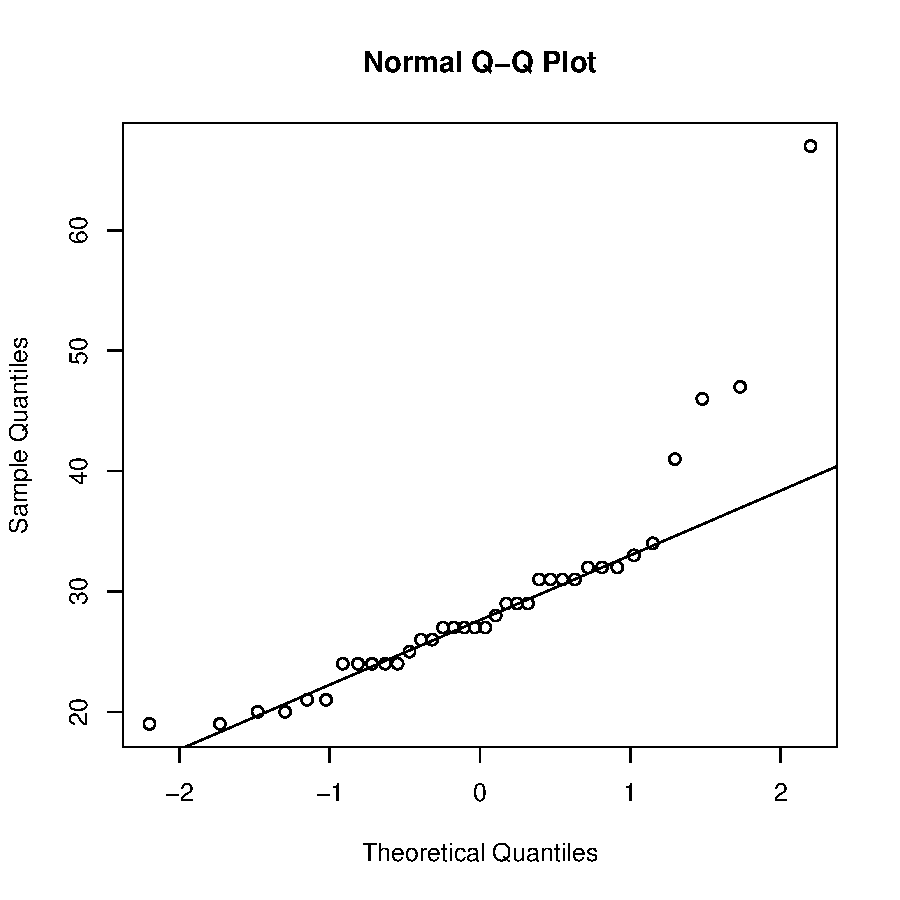
\includegraphics{FinalProjectPingTimes-004}
\label{residenceNorm}
\end{figure}

\begin{figure}
\centering
\caption{QQNorm compared with normal line of the data at the Oak Street residence}
\begin{Schunk}
\begin{Sinput}
> qqnorm(KalamazooCollege)
> qqline(KalamazooCollege)
\end{Sinput}
\end{Schunk}
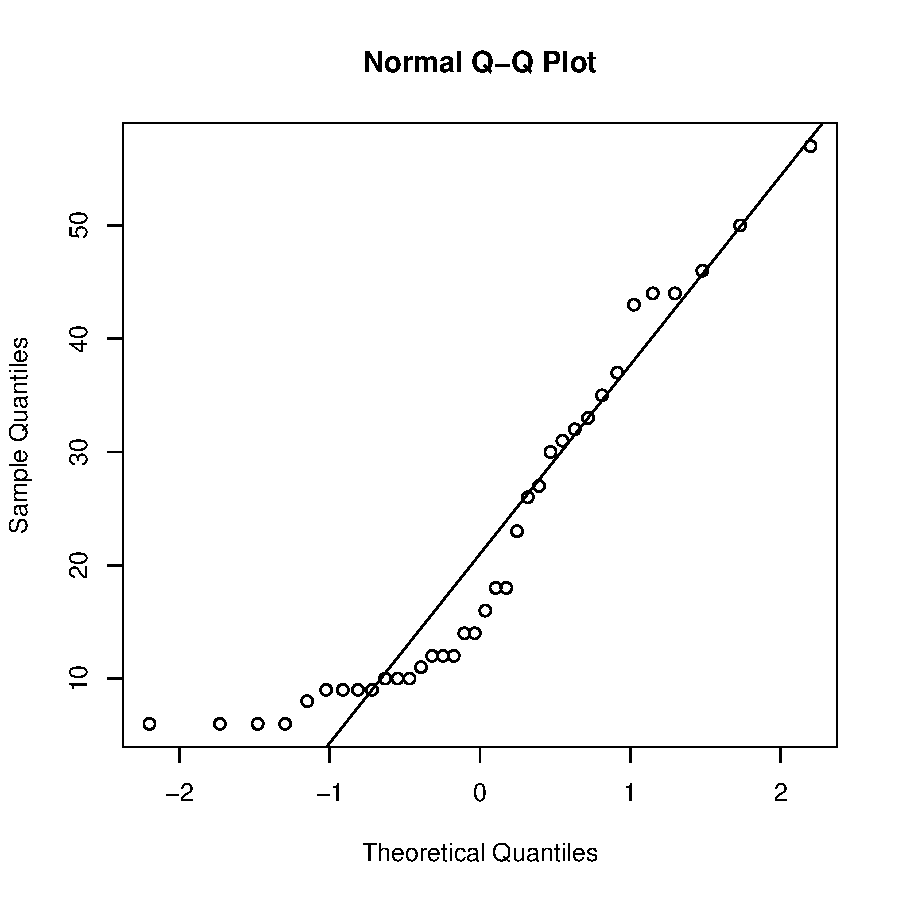
\includegraphics{FinalProjectPingTimes-005}
\label{kzooNorm}
\end{figure}


We see a difference in the sample means in figures \ref{kzooSum} and \ref{oakSum} . We then performed a bootstrap T test to see if the results are statistically significant.
\begin{figure}
\centering
\caption{Kalamazoo College}
\begin{Schunk}
\begin{Sinput}
> summary(KalamazooCollege)
\end{Sinput}
\begin{Soutput}
   Min. 1st Qu.  Median    Mean 3rd Qu.    Max. 
   6.00    9.75   15.00   21.75   32.25   57.00 
\end{Soutput}
\end{Schunk}
\label{kzooSum}
\end{figure}
\begin{figure}
\centering
\caption{Personal Residence Data}
\begin{Schunk}
\begin{Sinput}
> summary(PersonalResidence)
\end{Sinput}
\begin{Soutput}
   Min. 1st Qu.  Median    Mean 3rd Qu.    Max. 
  19.00   24.00   27.00   29.31   31.25   67.00 
\end{Soutput}
\end{Schunk}
\label{oakSum}
\end{figure}

\begin{Schunk}
\begin{Soutput}
[1] 0.0098
\end{Soutput}
\end{Schunk}

Since our p-value is less than .05, the difference in means is statistically significant at 95\% confidence. Given statistical significant of the difference in means we then found a confidence interval for $\mu$. For our confidence interval we bootstrap our quantiles. Metrics in our estimator are in figure \ref{stuff}.

\begin{figure}
\caption{Properties of the Bootstrapped difference in means}
\begin{Schunk}
\begin{Sinput}
> obs
\end{Sinput}
\begin{Soutput}
[1] -7.555556
\end{Soutput}
\begin{Sinput}
> bias
\end{Sinput}
\begin{Soutput}
[1] -0.0002722222
\end{Soutput}
\begin{Sinput}
> variance
\end{Sinput}
\begin{Soutput}
[1] 8.305899
\end{Soutput}
\begin{Sinput}
> #mean squared error
> variance - bias^2
\end{Sinput}
\begin{Soutput}
[1] 8.305899
\end{Soutput}
\begin{Sinput}
> quantile(times.diff.mean,c(0.025,0.975))
\end{Sinput}
\begin{Soutput}
      2.5%      97.5% 
-13.138889  -1.888889 
\end{Soutput}
\end{Schunk}
\ref{stuff}
\end{figure}

We find our 95\% confidence interval to be in support of our hypothesis that the true difference in means is nonzero. Because $H_0: \mu_{kzoo} = \mu_{oak}$  is not contained in the confidence interval we reject the null hypothesis and accept $H_A: \mu_{kzoo} \ne \mu_{oak}$. We use the bootstrapped sample means as a hypothesis for the true mean.

\section{Conclusion}
We conclude that Kalamazoo college's internet has lower latency as measured by ping than the Oak Street residence and that theoretically that there is a chance that the two networks are on different underlying connections. To confirm this, we traced a packet as it went from Kalamazoo College and the Oak Street residence to google. In figures 8 and 9 we see that a packet going to google.com consistently took a separate path. Furthermore, running the packet trace utility showed that Kalamazoo College and the Oak Street residence were running on different ISPs.
\begin{figure}
    \centering
    \begin{minipage}{.45\textwidth}
        \centering
        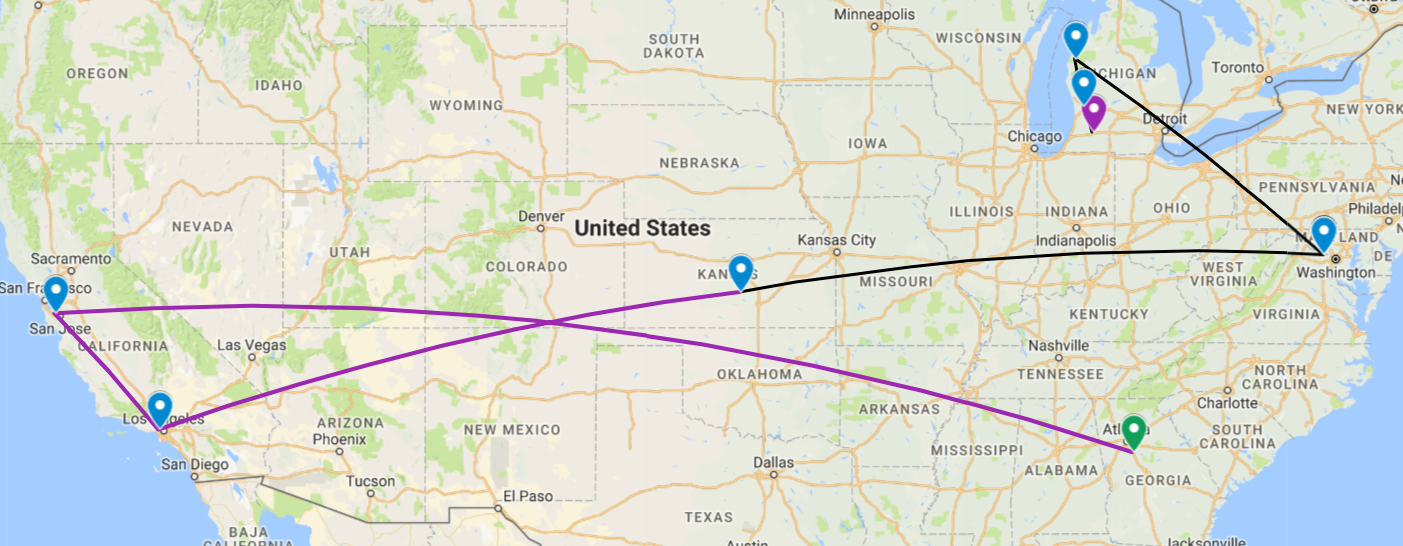
\includegraphics[width=\linewidth, height=0.15\textheight]{NetworkMapHome2.png}
        \caption{Packet network trace, Kalamazoo College to Google}
        \label{fig:prob1_6_2}
    \end{minipage}%
    \hspace{0.05\linewidth}
    \begin{minipage}{0.45\textwidth}
        \centering
        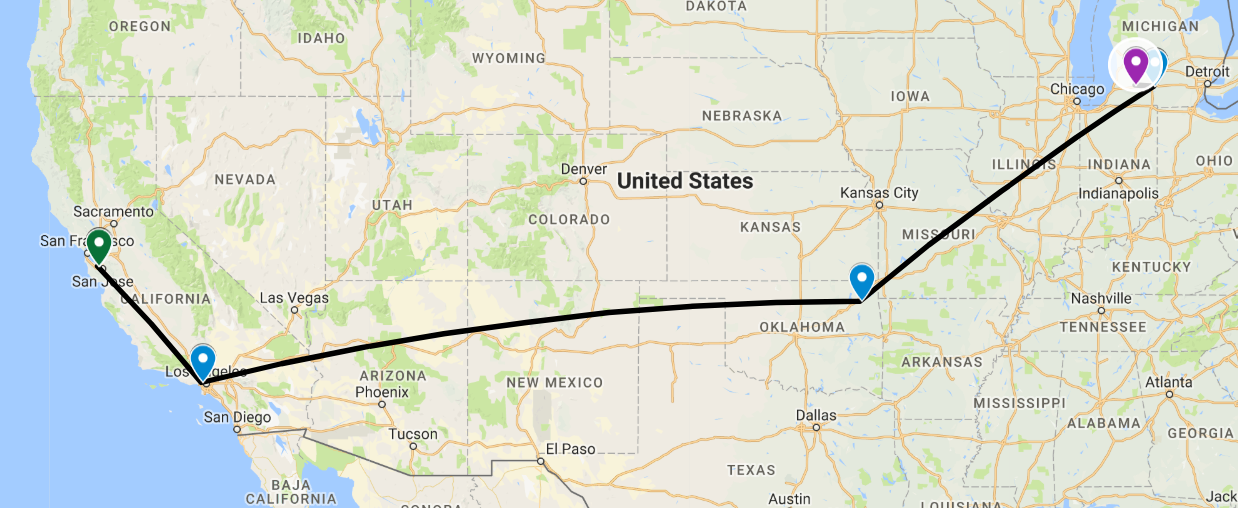
\includegraphics[width=\linewidth, height=0.15\textheight]{NetworkMapSchool.png}
        \caption{Network packet trace graph, 416 Oak St to Google}
        \label{fig:prob1_6_1}
    \end{minipage}
\end{figure}
\end{document}
